\documentclass[nooutcomes,noauthor,handout]{ximera}

\graphicspath{  
{./}
{./whoAreYou/}
{./drawingWithTheTurtle/}
{./bisectionMethod/}
{./circles/}
{./anglesAndRightTriangles/}
{./lawOfSines/}
{./lawOfCosines/}
{./plotter/}
{./staircases/}
{./pitch/}
{./qualityControl/}
{./symmetry/}
{./nGonBlock/}
}


%% page layout
\usepackage[cm,headings]{fullpage}
\raggedright
\setlength\headheight{13.6pt}


%% fonts
\usepackage{euler}

\usepackage{FiraMono}
\renewcommand\familydefault{\ttdefault} 
\usepackage[defaultmathsizes]{mathastext}
\usepackage[htt]{hyphenat}

\usepackage[T1]{fontenc}
\usepackage[scaled=1]{FiraSans}

%\usepackage{wedn}
\usepackage{pbsi} %% Answer font


\usepackage{cancel} %% strike through in pitch/pitch.tex


%% \usepackage{ulem} %% 
%% \renewcommand{\ULthickness}{2pt}% changes underline thickness

\tikzset{>=stealth}

\usepackage{adjustbox}

\setcounter{titlenumber}{-1}

%% journal style
\makeatletter
\newcommand\journalstyle{%
  \def\activitystyle{activity-chapter}
  \def\maketitle{%
    \addtocounter{titlenumber}{1}%
                {\flushleft\small\sffamily\bfseries\@pretitle\par\vspace{-1.5em}}%
                {\flushleft\LARGE\sffamily\bfseries\thetitlenumber\hspace{1em}\@title \par }%
                {\vskip .6em\noindent\textit\theabstract\setcounter{question}{0}\setcounter{sectiontitlenumber}{0}}%
                    \par\vspace{2em}
                    \phantomsection\addcontentsline{toc}{section}{\thetitlenumber\hspace{1em}\textbf{\@title}}%
                     }}
\makeatother



%% thm like environments
\let\question\relax
\let\endquestion\relax

\newtheoremstyle{QuestionStyle}{\topsep}{\topsep}%%% space between body and thm
		{}                      %%% Thm body font
		{}                              %%% Indent amount (empty = no indent)
		{\bfseries}            %%% Thm head font
		{)}                              %%% Punctuation after thm head
		{ }                           %%% Space after thm head
		{\thmnumber{#2}\thmnote{ \bfseries(#3)}}%%% Thm head spec
\theoremstyle{QuestionStyle}
\newtheorem{question}{}



\let\freeResponse\relax
\let\endfreeResponse\relax

%% \newtheoremstyle{ResponseStyle}{\topsep}{\topsep}%%% space between body and thm
%% 		{\wedn\bfseries}                      %%% Thm body font
%% 		{}                              %%% Indent amount (empty = no indent)
%% 		{\wedn\bfseries}            %%% Thm head font
%% 		{}                              %%% Punctuation after thm head
%% 		{3ex}                           %%% Space after thm head
%% 		{\underline{\underline{\thmname{#1}}}}%%% Thm head spec
%% \theoremstyle{ResponseStyle}

\usepackage[tikz]{mdframed}
\mdfdefinestyle{ResponseStyle}{leftmargin=1cm,linecolor=black,roundcorner=5pt,
, font=\bsifamily,}%font=\wedn\bfseries\upshape,}


\ifhandout
\NewEnviron{freeResponse}{}
\else
%\newtheorem{freeResponse}{Response:}
\newenvironment{freeResponse}{\begin{mdframed}[style=ResponseStyle]}{\end{mdframed}}
\fi



%% attempting to automate outcomes.

%% \newwrite\outcomefile
%%   \immediate\openout\outcomefile=\jobname.oc
%% \renewcommand{\outcome}[1]{\edef\theoutcomes{\theoutcomes #1~}%
%% \immediate\write\outcomefile{\unexpanded{\outcome}{#1}}}

%% \newcommand{\outcomelist}{\begin{itemize}\theoutcomes\end{itemize}}

%% \NewEnviron{listOutcomes}{\small\sffamily
%% After answering the following questions, students should be able to:
%% \begin{itemize}
%% \BODY
%% \end{itemize}
%% }
\usepackage[tikz]{mdframed}
\mdfdefinestyle{OutcomeStyle}{leftmargin=2cm,rightmargin=2cm,linecolor=black,roundcorner=5pt,
, font=\small\sffamily,}%font=\wedn\bfseries\upshape,}
\newenvironment{listOutcomes}{\begin{mdframed}[style=OutcomeStyle]After answering the following questions, students should be able to:\begin{itemize}}{\end{itemize}\end{mdframed}}



%% my commands

\newcommand{\snap}{{\bfseries\itshape\textsf{Snap!}}}
\newcommand{\flavor}{\link[\snap]{https://snap.berkeley.edu/}}
\newcommand{\mooculus}{\textsf{\textbf{MOOC}\textnormal{\textsf{ULUS}}}}


\usepackage{tkz-euclide}
\tikzstyle geometryDiagrams=[rounded corners=.5pt,ultra thick,color=black]
\colorlet{penColor}{black} % Color of a curve in a plot



\ifhandout\newcommand{\mynewpage}{\newpage}\else\newcommand{\mynewpage}{}\fi

\title{Rep-tiles and area}

\author{Bart Snapp}

\begin{document}
\begin{abstract}
  We will investigate more interesting rep-tiles.
\end{abstract}
\maketitle


\begin{listOutcomes}
\item Demonstrate given shapes are rep-$n$-tiles.
\item Recognize a relationship between scaling, perimeter, and area.
\end{listOutcomes}



Figuring out \textbf{how} shapes are rep-tiles can be difficult if
you don't actually have physical copies of the rep-tiles to play with.
I suggest you have someone help you write a \snap\ script using the block:
\begin{center}
  
\includegraphics{BLOCKreptile.png}
\end{center}
I'll explain the arguments (blanks in the BLOCK) for completeness sake.
Working \textbf{right-to-left,}
\begin{itemize}
\item the first TURTLE BLANK is for a costume,
\item the second TURTLE BLANK is for a horizontal reflection of the
  costume,
\item the blank labeled $r:$ is the size of the rotation in degrees, and
\item the blank labeled $w:$ is the desired width of the rep-tile.
\end{itemize}
To show a shape is a rep-tile, we have some keyboard commands.
\begin{itemize}
\item The ARROW keys will move the rep-tile around,
\item Pressing $r$ will rotate the rep-tile clockwise the specified
  number of degrees,
\item Pressing $f$ will flip the turtle horizontally across a line
  perpendicular to its base, and 
\item Pressing the SPACE-BAR will STAMP the rep-tile on the STAGE.
\end{itemize}


\mynewpage

\begin{question}
Consider the following polygons:
\[
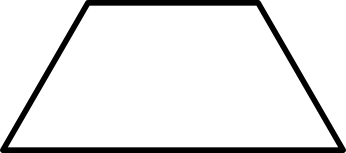
\includegraphics[width=.2\textwidth]{rhomb.png} \qquad
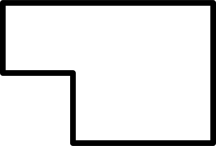
\includegraphics[width=.15\textwidth]{P.png}\qquad
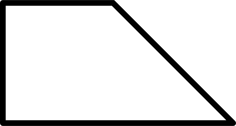
\includegraphics[width=.2\textwidth]{wedge.png} 
\]
Use the REPTILE BLOCK to show that each of these polygons is a
rep-$4$-tile. A SCREENSHOT of the \snap\ STAGE is sufficient.
\begin{freeResponse}
  \begin{itemize}
  \item Behold:
    \begin{center}
      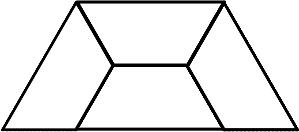
\includegraphics[width=.4\textwidth]{STAGErhomb.png}
    \end{center}
  \item Behold:
    \begin{center}
      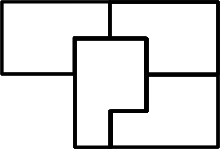
\includegraphics[width=.3\textwidth]{STAGEp.png}
    \end{center}
  \item Behold:
    \begin{center}
      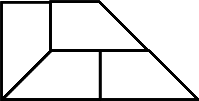
\includegraphics[width=.4\textwidth]{STAGEwedge.png}
    \end{center}
  \end{itemize}
\end{freeResponse}
\end{question}

\mynewpage


\begin{question}
  Now we'll investigate a rep-$4$-tile and a rep-$5$-tile.
  \begin{enumerate}
  \item Show that the following polygon is a rep-$4$-tile:
    \begin{center}
      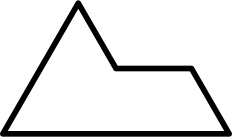
\includegraphics[width=.2\textwidth]{sphinx.png}
    \end{center}
  \item Show that a $(1,2,\sqrt{5})$ right triangle is a
    rep-$5$-tile.
    \begin{hint}
      I suggest you rotate $90^\circ$.
    \end{hint}
  \end{enumerate}
  In each case, if you want to convince me that you have a rep-tile,
  you must EXPLAIN why the angles are unchanged, and why the
  proportions of the linear measurements are unchanged.
  \begin{freeResponse}
    \begin{enumerate}
    \item Behold:
      \begin{center}
        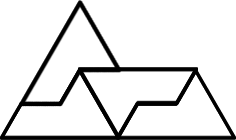
\includegraphics[width=.4\textwidth]{STAGEsphinx.png}
      \end{center}
      Let's call this polygon the ``sphinx.'' The sphinx has $3$ short
      sides say of length $1$, a longer side of length $2$, and a
      longest side of length $3$. The LARGER sphinx has short sides of
      length $2$, longer sides of length $4$, and longest sides of
      length $6$. We see that all the angles and proportions are the
      same.
    \item Behold:
      \begin{center}
        \begin{tikzpicture}[geometryDiagrams]
          \coordinate (A) at (0,0);
          \coordinate (B) at (4,2);
          \coordinate (C) at (4,0);
          \coordinate (BB) at (8,2);
          \coordinate (CC) at (8,0);
          \coordinate (BBB) at (8,4);
          \coordinate (D) at (10,0);
          
          \tkzDrawSegment (A,B)
          \tkzDrawSegment (A,C)
          \tkzDrawSegment (C,B)
          \tkzLabelSegment[above left](A,B){$\sqrt{5}$}
          \tkzLabelSegment[below](A,C){$2$}
          \tkzLabelSegment[right](B,C){$1$}  
          
          \tkzMarkAngle[size=1.5cm,thin,mark=](C,A,B)
          \tkzLabelAngle[pos=1.2](C,A,B){$\alpha$}
          
          \tkzMarkAngle[size=0.8cm,thin,mark=](A,B,C)
          \tkzLabelAngle[pos=.5](A,B,C){$\beta$}
          
          
          \tkzMarkRightAngle[thin](B,C,A)
          
          
          \tkzDrawSegment (C,BB)
          \tkzDrawSegment (BB,CC)
          \tkzDrawSegment (CC,C)
          \tkzLabelSegment[above left](C,BB){$\sqrt{5}$}
          \tkzLabelSegment[below](C,CC){$2$}
          \tkzLabelSegment[right](BB,CC){$1$}  
          
          \tkzMarkAngle[size=1.5cm,thin,mark=](CC,C,BB)
          \tkzLabelAngle[pos=1.2](CC,C,BB){$\alpha$}
          
          \tkzMarkAngle[size=0.8cm,thin,mark=](C,BB,CC)
          \tkzLabelAngle[pos=.5](C,BB,CC){$\beta$}
          
          
          \tkzMarkRightAngle[thin](BB,CC,C)
          

          
          
          \tkzDrawSegment (BBB,B)
          \tkzDrawSegment (BBB,BB)
          \tkzDrawSegment (B,BB)
          \tkzLabelSegment[above left](B,BBB){$\sqrt{5}$}
          \tkzLabelSegment[below](B,BB){$2$}
          \tkzLabelSegment[left](BB,BBB){$1$}  
          
          \tkzMarkAngle[size=1.5cm,thin,mark=](BB,B,BBB)
          \tkzLabelAngle[pos=1.2](BB,B,BBB){$\alpha$}
          
          \tkzMarkAngle[size=0.8cm,thin,mark=](B,BBB,BB)
          \tkzLabelAngle[pos=.5](B,BBB,BB){$\beta$}
          
          \tkzMarkRightAngle[thin](BBB,BB,B)
          



          \tkzMarkAngle[size=1.5cm,thin,mark=](B,BB,C)
          \tkzLabelAngle[pos=1.2](B,BB,C){$\alpha$}
          
          \tkzMarkAngle[size=0.8cm,thin,mark=](BB,C,B)
          \tkzLabelAngle[pos=.5](BB,C,B){$\beta$}
         
          \tkzMarkRightAngle[thin](C,B,BB)



          \tkzDrawSegment (D,CC)
          \tkzDrawSegment (D,BBB)
          \tkzLabelSegment[right](D,BBB){$\sqrt{5}$}
          \tkzLabelSegment[below](D,CC){$1$}  
          
          \tkzMarkAngle[size=1.5cm,thin,mark=](CC,BBB,D)
          \tkzLabelAngle[pos=1.2](CC,BBB,D){$\alpha$}
          
          \tkzMarkAngle[size=0.8cm,thin,mark=](BBB,D,CC)
          \tkzLabelAngle[pos=.5](BBB,D,CC){$\beta$}
          
          
          \tkzMarkRightAngle[thin](D,CC,BBB)
        \end{tikzpicture}
      \end{center}
      Since $\alpha+\beta+90^\circ = 180^\circ$, We see that all the angles of the
      larger figure are the same as our starting $(1,2,\sqrt{5})$
      right triangle. Also we see
      \begin{align*}
        \frac{\text{long leg}}{\text{short leg}} &= \frac{2}{1} = \frac{\sqrt{5}+\sqrt{5}}{\sqrt{5}},\\
        \frac{\text{hypotenuse}}{\text{short leg}} &= \frac{\sqrt{5}}{1} = \frac{5}{\sqrt{5}},\\
        \frac{\text{hypotenuse}}{\text{long leg}} &= \frac{\sqrt{5}}{2} = \frac{5}{2\sqrt{5}}.\\
      \end{align*}
    \end{enumerate}
  \end{freeResponse}
\end{question}

\mynewpage

\begin{question}
  Now we'll connect rep-tiles to SCALING area.
  \begin{enumerate}
  \item Fill-in the table:
    \[
    \renewcommand{\arraystretch}{3}
    \begin{array}{|c||c|}
      \hline
          \text{rep-$n$-tile} &  \frac{\text{new area}}{\text{old area}}  \\
          \hline\hline
          2 &     \\  \hline
          3 &      \\ \hline
          4 &      \\ \hline
          5 &      \\\hline 
        \end{array}
    \]
    \item Based ON OUR PREVIOUS EXAMPLES, make your BEST GUESSES to
      complete the table below:
        \[
    \renewcommand{\arraystretch}{3}
    \begin{array}{|c||c|}
      \hline
          \text{rep-$n$-tile} &  \frac{\text{new perimeter}}{\text{old perimeter}}  \\
          \hline\hline
          2 &     \\  \hline
          3 &     \\ \hline
          4 &      \\ \hline
          5 &      \\\hline 
        \end{array}
    \]
  \end{enumerate}
  \begin{freeResponse}
    \begin{enumerate}
    \item Behold:
      \[
      \renewcommand{\arraystretch}{3}
      \begin{array}{|c||c|}
        \hline
        \text{rep-$n$-tile} &  \frac{\text{new area}}{\text{old area}}  \\
        \hline\hline
        2 &  2  \\  \hline
        3 &  3   \\ \hline
        4 &  4   \\ \hline
        5 &  5   \\\hline 
      \end{array}
      \]
    \item Behold:
      \[
      \renewcommand{\arraystretch}{3}
      \begin{array}{|c||c|}
      \hline
      \text{rep-$n$-tile} &  \frac{\text{new perimeter}}{\text{old perimeter}}  \\
      \hline\hline
      2 & \sqrt{2}  \\  \hline
      3 & \sqrt{3}  \\ \hline
      4 & 2         \\ \hline
      5 &  \sqrt{5} \\\hline 
      \end{array}
      \]
    \end{enumerate}
  \end{freeResponse}
\end{question}
\end{document}
